\documentclass[20pt,a1paper,landscape]{tikzposter}

% required packages
\usepackage{amsmath}
\usepackage{amsfonts}
\usepackage{amsthm}
\usepackage{tikz}
\usepackage{graphicx}
\usepackage{natbib}

% compact bibliography
\renewcommand{\bibsection}{}
\setlength{\bibsep}{0pt plus 0.3ex}

% tiks fun
\usetikzlibrary{shapes,decorations,arrows,calc,arrows.meta,fit,positioning}
\tikzset{
    -Latex,auto,node distance =1 cm and 1 cm,semithick,
    state/.style ={ellipse, draw, minimum width = 1 cm},
    point/.style = {circle, draw, inner sep=0.1cm,fill,node contents={}},
    bidirected/.style={Latex-Latex,dashed},
    el/.style = {inner sep=2pt, align=left, sloped}
}

% set up new enumerate style for assumptions
\renewcommand{\labelenumi}{(A\arabic{enumi})}

% math macros
\newcommand{\D}{\mathcal{D}}
\newcommand{\E}{\mathbb{E}}
\newcommand{\F}{\mathcal{F}}
\newcommand{\M}{\mathcal{M}}
\newcommand{\R}{\mathbb{R}}
\newcommand{\X}{\mathcal{X}}
\newcommand{\logit}{\text{logit}}
\newcommand{\like}{\mathcal{L}}
\renewcommand{\P}{\mathbb{P}}
\newcommand{\I}{\mathbbm{I}}
\newcommand{\1}{\mathbbm{1}}
\newcommand{\indep}{\mbox{$\perp\!\!\!\perp$}}
\DeclareMathOperator*{\argmin}{\arg\!\min}
\DeclareMathOperator*{\argmax}{\arg\!\max}

%% Available themes: see also
%% https://bitbucket.org/surmann/tikzposter/downloads/themes.pdf
\usetheme{Default}
\colorlet{backgroundcolor}{white}

% title information
\title{Identifying Direct Causal Effects Under Unmeasured Confounding}
\author{Philippe Boileau$^{\ast 1}$, Nima S. Hejazi$^{\ast 2}$,
  Ivana Malenica$^{\ast 1}$, Sandrine Dudoit$^1$, Mark J. van der Laan$^1$}
\institute{$^1$University of California, Berkeley; $^2$Weill Cornell Medicine}
%\titlegraphic{}

% dictate default block options
\newcommand{\myblock}[2]{\block[titleinnersep=2mm, linewidth=0.5mm]{#1}{#2}}
\newcommand{\mysmallblock}[2]{\block[titleinnersep=1mm, linewidth=1mm, bodyinnersep=5mm, roundedcorners=12, ]{{\small #1}}{{\tiny#2\par}}}

\begin{document}

\maketitle[width = 26in]
\node[anchor=west] at (TP@title.west) {
\includegraphics[width=5cm]{logos/cal}};
\node[anchor=east] at (TP@title.east) {
\includegraphics[scale=0.7]{logos/wcm}};


\begin{columns}

  \column{0.333}

  \myblock{Introduction \& Motivations}{
    \begin{itemize}
      \itemsep2pt
        \item Developing \textit{mechanistic} understandings of causal effects
          is a ubiquitous goal across scientific disciplines.
        \item The natural direct and indirect effects are common target causal
          parameters since they are nonparametrically identified.
        \item Identification assumes absence of unmeasured confounders of
          exposure--mediator, mediator--outcome, and exposure--outcome
          pathways --- but this is \textit{not} completely necessary.
        \item The natural direct and indirect effects arise from a decomposition
          of the average treatment effect (ATE), and the
          \begin{itemize}
            \itemsep1pt
            \item natural indirect effect (NIE) captures the portion of the ATE
              passing through the mediators ($Z$), while the
            \item natural direct effect (NDE) captures the remainder of the ATE,
              through all paths excluding $Z$.
          \end{itemize}
    \end{itemize}
  }

  \myblock{The Statistical Problem}{
    %State the causal and statistical models, and estimand.
    Consider cohort data collected through time as $O = (W, A, Z, Y).$
    $O$ does not include $V$, the exposure--mediator confounder, though the
    complete data $X$ does. \\

    Let $O \sim P_0 \in \M$, with $\M$ being the nonparametric
    \textit{statistical model}. The likelihood of the observed data under $\M$
    is:
    \begin{equation*}
      p(o) = \prod_{i=1}^{n} q_Y(y_i \mid w_i, a_i, z_i) q_Z(z_i \mid w_i, a_i)
        g_A(a_i \mid w_i) q_W(w_i).
    \end{equation*}

    The average treatment effect may be decomposed as
    \begin{align*}
      \Psi_{\text{ATE}}^F(P_{U,X,0})
      %=& \E_{U,X,0}[Y(1) - Y(0)] \\
       =& \underbrace{\E_{U,X,0}[Y(1, Z(1)) - Y(1, Z(0))]}_{\text{NIE}} \\
       &+ \underbrace{\E_{U,X,0}[Y(1, Z(0)) - Y(0, Z(0))]}_{\text{NDE}},
    \end{align*}
    where $Y(1, Z(0))$ arises from a \textit{joint} intervention on treatment
    and mediators ($Z$), setting them to incompatible values. The NDE is
    \begin{align*}
      \Psi^F_{\text{NDE}}(P_{U,X,0}) &= \int_{\mathcal{W}, \mathcal{Z}}
        \E[Y(1,z) - Y(0,z) \mid W=w] \\
        & \qquad\qquad\qquad p_Z(z \mid A=0,w)p_W(w)~d\mu(z)~d\nu(w) \ .
    \end{align*}

    \vspace{-1em}
  }

  \column{0.334}

  \myblock{Causal Identification}{

    \centering
    \begin{tikzpicture}
      \node[state] (1) at (0,7.0) {$W$};
      \node[state] (2) at (0,4) {$Z$};
      \node[state,rectangle] (3) at (0,0) {$V$};
      \node[state] (4) at (-6,2) {$A$};
      \node[state] (5) at (6,2) {$Y$};

      \path (1) edge (2);
      \path (1) edge (5);
      \path (1) edge (4);

      \path (4) edge[densely dotted] (5);
      \path (4) edge[dashed] (2);
      \path (2) edge[dashed] (5);

      \path (3) edge (4);
      \path (3) edge (2);

      \node[draw=red,loosely dotted,fit=(3) (5), inner sep=0.2cm,line width=0.05cm] (machine) {};
    \end{tikzpicture}

    \begin{enumerate}
      \item No unmeasured endogenous pathways:\newline
        $f_Y(Z, A, W, V, U_Y) \equiv f_Y(Z, A, W, U_Y).$
      \item Conditional expectation equivalence:\newline
        $\E(Y \mid Z,A=1,W,V) \equiv \E(Y \mid Z,A=1,W)$
    \end{enumerate}

    \innerblock[]{Theorem}{
      Under assumptions A1 and A2, $\Psi^F_{\text{NDE}}(P_{U,X,0})$ is
      identified by
      \begin{align*}
        \Psi(P_0)
        &= \E_{P_0}\E_{P_0} \{\E_{P_0}(Y \mid W,A=1,Z) \\
        &\qquad\qquad\qquad - \E_{P_0}(Y \mid W,A=0,Z) \mid A=0,W\} \ .
      \end{align*}
    }
  }

  \myblock{Inference}{

    \textbf{Existing estimation and testing approaches are compatible with
    this relaxed identification strategy.} For example,
    \begin{itemize}
      \itemsep0pt
      \item targeted maximum likelihood estimator of~\citet{zheng2012}
      \item one-step bias-corrected estimator based on the efficient influence
        function of \citet{tchetgen2011}.
    \end{itemize}
    Both estimators are \textit{multiple-robust}, \textit{asymptotically linear} under fairly
    non-restrictive assumptions, and compatible with cross-fitting.\\
    Both estimators are implemented in the \texttt{medoutcon} \texttt{R}
    package.
  }

  \mysmallblock{Funding}{
    PB's gratefully acknowledges the support of the FRQNT and NSERC. NSH's work
    was supported by NSF DMS 2102840.
  }

  \column{0.333}

  \myblock{Numerical Experiments}{

    We consider the following data-generating process:
    \begin{align*}\label{eq:nde-sim-dgp}
      W_1 & \sim \text{Unif}(-1, 1); \: W_2, V \sim \text{Norm}(0, 1) \\
      A|W, V & \sim \text{Bern}
      \left(\left(1 + \exp\{-W_1-W_2-V\}\right)^{-1}\right) \\
      Z|A, W, V & \sim \text{Bern}
      \left(\left(1 + \exp\{-W_1-W_2- \gamma V - 3A\}\right)^{-1}\right) \\
      Y| Z, A, W, V & \sim \text{Norm}(3A + W_1 + W_2 + Z, 1) \ .
    \end{align*}
    \centering

    \vspace{-2em}

    \begin{tikzfigure}
      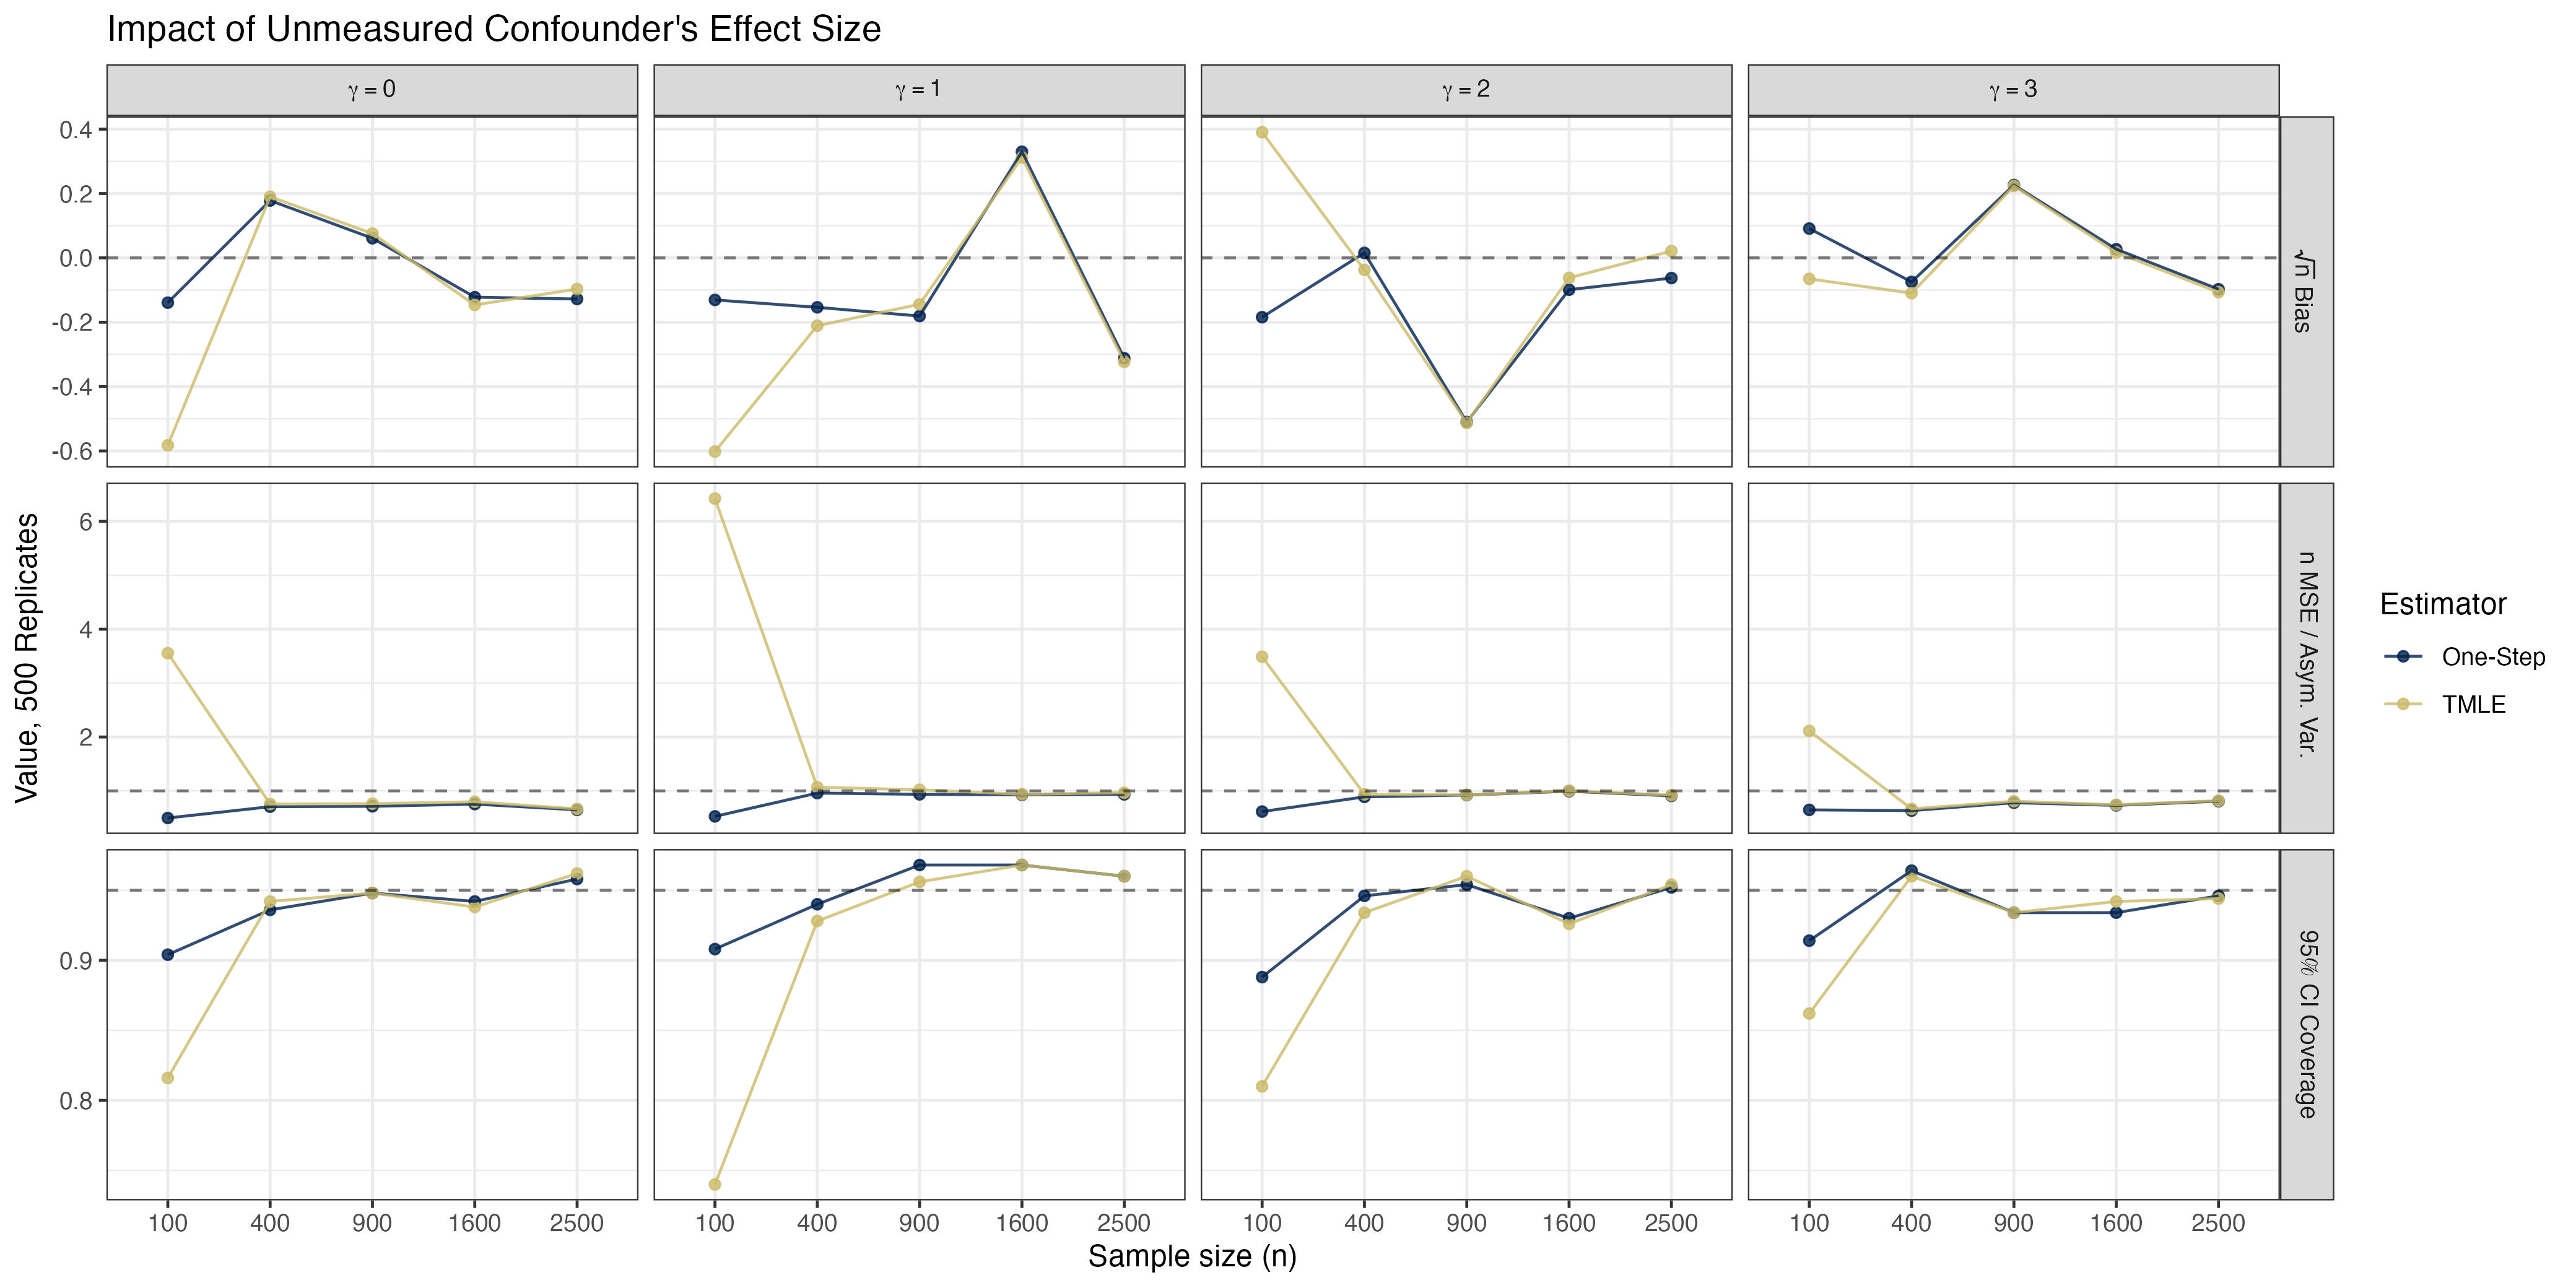
\includegraphics[width=0.295\textwidth]{figs/impact-unmeasured-conf-eff-size-sim.jpeg}
    \end{tikzfigure}
    \vspace{-2em}
  }

  \myblock{Conclusions}{
    \vspace{-1em}
    \begin{itemize}
      \itemsep1pt
        \item The NDE is identifiable under unmeasured exposure--mediator
          confounding by a \textit{well-studied} statistical functional!
        \item The NDE has recently been used to study the \textit{proportion of
          vaccine effect mediated} through candidate immune correlates.
          \begin{itemize}
            \itemsep0pt
            \item Our results strengthen ``out-of-the-box'' uses of the NDE.
            \item Exposure--mediator confounders in vaccine studies: prior
              infection history, immunocompromised status, genetics.
          \end{itemize}
    \end{itemize}
    \vspace{-1.5em}
  }

  \mysmallblock{References}{
    \vspace{-3em}
    \bibliographystyle{unsrtnat}
    \bibliography{refs}
    \vspace{-1em}
  }

  \begin{subcolumns}
    \subcolumn{0.7}
    \block[linewidth=0mm, bodyinnersep=5mm, roundedcorners=12]{}{
      \vspace{-0.5em}
      {\small \textit{$^\ast$ indicates shared first-authorship, ordered
      alphabetically.}}
      \vspace{-1em}
    }
  \end{subcolumns}


\end{columns}

\end{document}
